\documentclass[10pt,compress,t,notes=noshow, xcolor=table]{beamer}
\newcommand{\btVFill}{\vskip0pt plus 1filll}
\newcommand\hmmax{0}
\newcommand\bmmax{0}
\usepackage[]{graphicx}
% graphicx is loaded via lmu-lecture.sty as well
\usepackage[]{color}
% maxwidth is the original width if it is less than linewidth
% otherwise use linewidth (to make sure the graphics do not exceed the margin)
\makeatletter
\def\maxwidth{ %
  \ifdim\Gin@nat@width>\linewidth
    \linewidth
  \else
    \Gin@nat@width
  \fi
}
\makeatother

% ---------------------------------%
% latex-math dependencies, do not remove:
% - mathtools
% - bm
% - siunitx
% - dsfont
% - xspace
% ---------------------------------%

%--------------------------------------------------------%
%       Language, encoding, typography
%--------------------------------------------------------%

\usepackage[english]{babel}
\usepackage[utf8]{inputenc} % Enables inputting UTF-8 symbols
% Standard AMS suite (loaded via lmu-lecture.sty)
\usepackage{amsmath,amsfonts,amssymb}

% Font for double-stroke / blackboard letters for sets of numbers (N, R, ...)
% Distribution name is "doublestroke"
% According to https://mirror.physik.tu-berlin.de/pub/CTAN/fonts/doublestroke/dsdoc.pdf
% the "bbm" package does a similar thing and may be superfluous.
% Required for latex-math
\usepackage{dsfont}

% bbm – "Blackboard-style" cm fonts (https://www.ctan.org/pkg/bbm)
% Used to be in common.tex, loaded directly after this file
% Maybe superfluous given dsfont is loaded
% TODO: Check if really unused?
% \usepackage{bbm}

% bm – Access bold symbols in maths mode - https://ctan.org/pkg/bm
% Required for latex-math, preferred over \boldsymbol
% https://tex.stackexchange.com/questions/3238/bm-package-versus-boldsymbol
\usepackage{bm}

% pifont – Access to PostScript standard Symbol and Dingbats fonts
% Used for \newcommand{\xmark}{\ding{55}, which is never used
% aside from lecture_advml/attic/xx-automl/slides.Rnw
% \usepackage{pifont}

% Quotes (inline and display), provdes \enquote
% https://ctan.org/pkg/csquotes
\usepackage{csquotes}

% Adds arg to enumerate env, technically superseded by enumitem according
% to https://ctan.org/pkg/enumerate
% Replace with https://ctan.org/pkg/enumitem ?
% Even better: enumitem is not really compatible with beamer and breaks all sorts of things
% particularly the enumerate environment. The enumerate package also just isn't required
% from what I can tell so... don't re-add it I guess?
% \usepackage{enumerate}

% Line spacing - provides \singlespacing \doublespacing \onehalfspacing
% https://ctan.org/pkg/setspace
% \usepackage{setspace}

% mathtools – Mathematical tools to use with amsmath
% https://ctan.org/pkg/mathtools?lang=en
% latex-math dependency according to latex-math repo
\usepackage{mathtools}

% Maybe not great to use this https://tex.stackexchange.com/a/197/19093
% Use align instead -- TODO: Global search & replace to check, eqnarray is used a lot
% $ rg -f -u "\begin{eqnarray" -l | grep -v attic | awk -F '/' '{print $1}' | sort | uniq -c
%   13 lecture_advml
%   14 lecture_i2ml
%    2 lecture_iml
%   27 lecture_optimization
%   45 lecture_sl
\usepackage{eqnarray}

% For shaded regions / boxes
% Used sometimes in optim
% https://www.ctan.org/pkg/framed
\usepackage{framed}

%--------------------------------------------------------%
%       Cite button (version 2024-05)
%--------------------------------------------------------%
% Note this requires biber to be in $PATH when running,
% telltale error in log would be e.g. Package biblatex Info: ... file 'authoryear.dbx' not found
% aside from obvious "biber: command not found" or similar.
% Tried moving this to lmu-lecture.sty but had issues I didn't quite understood,
% so it's here for now.

\usepackage{textcase} % for \NoCaseChange
\usepackage{hyperref}

% Only try adding a references file if it exists, otherwise
% this would compile error when references.bib is not found
\IfFileExists{references.bib} {
  \usepackage{usebib}
  \usepackage[backend=biber, style=authoryear]{biblatex}

  \addbibresource{./references.bib}
  \bibinput{references}
}

\newcommand{\citelink}[1]{%
\NoCaseChange{\resizebox{!}{9pt}{\protect\beamergotobutton{\href{\usebibentry{\NoCaseChange{#1}}{url}}{\begin{NoHyper}\cite{#1}\end{NoHyper}}}}}%
}

%--------------------------------------------------------%
%       Displaying code and algorithms
%--------------------------------------------------------%

% Reimplements verbatim environments: https://ctan.org/pkg/verbatim
% verbatim used sed at least once in
% supervised-classification/slides-classification-tasks.tex
% Removed since code should not be put on slides anyway
% \usepackage{verbatim}

% Both used together for algorithm typesetting, see also overleaf: https://www.overleaf.com/learn/latex/Algorithms
% algorithmic env is also used, but part of the bundle:
%   "algpseudocode is part of the algorithmicx bundle, it gives you an improved version of algorithmic besides providing some other features"
% According to https://tex.stackexchange.com/questions/229355/algorithm-algorithmic-algorithmicx-algorithm2e-algpseudocode-confused
\usepackage{algorithm}
\usepackage{algpseudocode}

%--------------------------------------------------------%
%       Tables
%--------------------------------------------------------%

% multi-row table cells: https://www.namsu.de/Extra/pakete/Multirow.html
% Provides \multirow
% Used e.g. in evaluation/slides-evaluation-measures-classification.tex
\usepackage{multirow}

% colortbl: https://ctan.org/pkg/colortbl
% "The package allows rows and columns to be coloured, and even individual cells." well.
% Provides \columncolor and \rowcolor
% \rowcolor is used multiple times, e.g. in knn/slides-knn.tex
\usepackage{colortbl}

% long/multi-page tables: https://texdoc.org/serve/longtable.pdf/0
% Not used in slides
% \usepackage{longtable}

% pretty table env: https://ctan.org/pkg/booktabs
% Is used
% Defines \toprule
\usepackage{booktabs}

%--------------------------------------------------------%
%       Figures: Creating, placing, verbing
%--------------------------------------------------------%

% wrapfig - Wrapping text around figures https://de.overleaf.com/learn/latex/Wrapping_text_around_figures
% Provides wrapfigure environment -used in lecture_optimization
\usepackage{wrapfig}

% Sub figures in figures and tables
% https://ctan.org/pkg/subfig -- supersedes subfigure package
% Provides \subfigure
% \subfigure not used in slides but slides-tuning-practical.pdf errors without this pkg, error due to \captionsetup undefined
\usepackage{subfig}

% Actually it's pronounced PGF https://en.wikibooks.org/wiki/LaTeX/PGF/TikZ
\usepackage{tikz}

% No idea what/why these settings are what they are but I assume they're there on purpose
\usetikzlibrary{shapes,arrows,automata,positioning,calc,chains,trees, shadows}
\tikzset{
  %Define standard arrow tip
  >=stealth',
  %Define style for boxes
  punkt/.style={
    rectangle,
    rounded corners,
    draw=black, very thick,
    text width=6.5em,
    minimum height=2em,
    text centered},
  % Define arrow style
  pil/.style={
    ->,
    thick,
    shorten <=2pt,
    shorten >=2pt,}
}

%--------------------------------------------------------%
%       Beamer setup and custom macros & environments
%--------------------------------------------------------%

% Main sty file for beamer setup (layout, style, lecture page numbering, etc.)
% For long-term maintenance, this may me refactored into a more modular set of .sty files
\usepackage{../../style/lmu-lecture}
% Custom itemize wrappers, itemizeS, itemizeL, etc
\usepackage{../../style/customitemize}
% Custom framei environment, uses custom itemize!
\usepackage{../../style/framei}
% Custom frame2 environment, allows specifying font size for all content
\usepackage{../../style/frame2}
% Column layout macros
\usepackage{../../style/splitV} 

% Used regularly
\let\code=\texttt

% Not sure what/why this does
\setkeys{Gin}{width=0.9\textwidth}

% -- knitr leftovers --
% Used often in conjunction with \definecolor{shadecolor}{rgb}{0.969, 0.969, 0.969}
% Removing definitions requires chaning _many many_ slides, which then need checking to see if output still ok
\definecolor{fgcolor}{rgb}{0.345, 0.345, 0.345}
\definecolor{shadecolor}{rgb}{0.969, 0.969, 0.969}
\newenvironment{knitrout}{}{} % an empty environment to be redefined in TeX

%-------------------------------------------------------------------------------------------------------%
%  Unused stuff that needs to go but is kept here currently juuuust in case it was important after all  %
%-------------------------------------------------------------------------------------------------------%

% \newcommand{\hlnum}[1]{\textcolor[rgb]{0.686,0.059,0.569}{#1}}%
% \newcommand{\hlstr}[1]{\textcolor[rgb]{0.192,0.494,0.8}{#1}}%
% \newcommand{\hlcom}[1]{\textcolor[rgb]{0.678,0.584,0.686}{\textit{#1}}}%
% \newcommand{\hlopt}[1]{\textcolor[rgb]{0,0,0}{#1}}%
% \newcommand{\hlstd}[1]{\textcolor[rgb]{0.345,0.345,0.345}{#1}}%
% \newcommand{\hlkwa}[1]{\textcolor[rgb]{0.161,0.373,0.58}{\textbf{#1}}}%
% \newcommand{\hlkwb}[1]{\textcolor[rgb]{0.69,0.353,0.396}{#1}}%
% \newcommand{\hlkwc}[1]{\textcolor[rgb]{0.333,0.667,0.333}{#1}}%
% \newcommand{\hlkwd}[1]{\textcolor[rgb]{0.737,0.353,0.396}{\textbf{#1}}}%
% \let\hlipl\hlkwb

% \makeatletter
% \newenvironment{kframe}{%
%  \def\at@end@of@kframe{}%
%  \ifinner\ifhmode%
%   \def\at@end@of@kframe{\end{minipage}}%
%   \begin{minipage}{\columnwidth}%
%  \fi\fi%
%  \def\FrameCommand##1{\hskip\@totalleftmargin \hskip-\fboxsep
%  \colorbox{shadecolor}{##1}\hskip-\fboxsep
%      % There is no \\@totalrightmargin, so:
%      \hskip-\linewidth \hskip-\@totalleftmargin \hskip\columnwidth}%
%  \MakeFramed {\advance\hsize-\width
%    \@totalleftmargin\z@ \linewidth\hsize
%    \@setminipage}}%
%  {\par\unskip\endMakeFramed%
%  \at@end@of@kframe}
% \makeatother

% \definecolor{shadecolor}{rgb}{.97, .97, .97}
% \definecolor{messagecolor}{rgb}{0, 0, 0}
% \definecolor{warningcolor}{rgb}{1, 0, 1}
% \definecolor{errorcolor}{rgb}{1, 0, 0}
% \newenvironment{knitrout}{}{} % an empty environment to be redefined in TeX

% \usepackage{alltt}
% \newcommand{\SweaveOpts}[1]{}  % do not interfere with LaTeX
% \newcommand{\SweaveInput}[1]{} % because they are not real TeX commands
% \newcommand{\Sexpr}[1]{}       % will only be parsed by R
% \newcommand{\xmark}{\ding{55}}%

% textpos – Place boxes at arbitrary positions on the LATEX page
% https://ctan.org/pkg/textpos
% Provides \begin{textblock}
% TODO: Check if really unused?
% \usepackage[absolute,overlay]{textpos}

% -----------------------%
% Likely knitr leftovers %
% -----------------------%

% psfrag – Replace strings in encapsulated PostScript figures
% https://www.overleaf.com/latex/examples/psfrag-example/tggxhgzwrzhn
% https://ftp.mpi-inf.mpg.de/pub/tex/mirror/ftp.dante.de/pub/tex/macros/latex/contrib/psfrag/pfgguide.pdf
% Can't tell if this is needed
% TODO: Check if really unused?
% \usepackage{psfrag}

% arydshln – Draw dash-lines in array/tabular
% https://www.ctan.org/pkg/arydshln
% !! "arydshln has to be loaded after array, longtable, colortab and/or colortbl"
% Provides \hdashline and \cdashline
% Not used in slides
% \usepackage{arydshln}

% tabularx – Tabulars with adjustable-width columns
% https://ctan.org/pkg/tabularx
% Provides \begin{tabularx}
% Not used in slides
% \usepackage{tabularx}

% placeins – Control float placement
% https://ctan.org/pkg/placeins
% Defines a \FloatBarrier command
% TODO: Check if really unused?
% \usepackage{placeins}

% Can't find a reason why common.tex is not just part of this file?
% This file is included in slides and exercises

% Rarely used fontstyle for R packages, used only in 
% - forests/slides-forests-benchmark.tex
% - exercises/single-exercises/methods_l_1.Rnw
% - slides/cart/attic/slides_extra_trees.Rnw
\newcommand{\pkg}[1]{{\fontseries{b}\selectfont #1}}

% Spacing helpers, used often (mostly in exercises for \dlz)
\newcommand{\lz}{\vspace{0.5cm}} % vertical space (used often in slides)
\newcommand{\dlz}{\vspace{1cm}}  % double vertical space (used often in exercises, never in slides)
\newcommand{\oneliner}[1] % Oneliner for important statements, used e.g. in iml, algods
{\begin{block}{}\begin{center}\begin{Large}#1\end{Large}\end{center}\end{block}}

% Don't know if this is used or needed, remove?
% textcolor that works in mathmode
% https://tex.stackexchange.com/a/261480
% Used e.g. in forests/slides-forests-bagging.tex
% [...] \textcolor{blue}{\tfrac{1}{M}\sum^M_{m} [...]
% \makeatletter
% \renewcommand*{\@textcolor}[3]{%
%   \protect\leavevmode
%   \begingroup
%     \color#1{#2}#3%
%   \endgroup
% }
% \makeatother


% dependencies: amsmath, amssymb, dsfont
% math spaces
\ifdefined\N
\renewcommand{\N}{\mathds{N}} % N, naturals
\else \newcommand{\N}{\mathds{N}} \fi
\newcommand{\Z}{\mathds{Z}} % Z, integers
\newcommand{\Q}{\mathds{Q}} % Q, rationals
\newcommand{\R}{\mathds{R}} % R, reals
\ifdefined\C
\renewcommand{\C}{\mathds{C}} % C, complex
\else \newcommand{\C}{\mathds{C}} \fi
\newcommand{\continuous}{\mathcal{C}} % C, space of continuous functions
\newcommand{\M}{\mathcal{M}} % machine numbers
\newcommand{\epsm}{\epsilon_m} % maximum error

% counting / finite sets
\newcommand{\setzo}{\{0, 1\}} % set 0, 1
\newcommand{\setmp}{\{-1, +1\}} % set -1, 1
\newcommand{\unitint}{[0, 1]} % unit interval

% basic math stuff
\newcommand{\xt}{\tilde x} % x tilde
\DeclareMathOperator*{\argmax}{arg\,max} % argmax
\DeclareMathOperator*{\argmin}{arg\,min} % argmin
\newcommand{\argminlim}{\mathop{\mathrm{arg\,min}}\limits} % argmax with limits
\newcommand{\argmaxlim}{\mathop{\mathrm{arg\,max}}\limits} % argmin with limits
\newcommand{\sign}{\operatorname{sign}} % sign, signum
\newcommand{\I}{\mathbb{I}} % I, indicator
\newcommand{\order}{\mathcal{O}} % O, order
\newcommand{\bigO}{\mathcal{O}} % Big-O Landau
\newcommand{\littleo}{{o}} % Little-o Landau
\newcommand{\pd}[2]{\frac{\partial{#1}}{\partial #2}} % partial derivative
\newcommand{\floorlr}[1]{\left\lfloor #1 \right\rfloor} % floor
\newcommand{\ceillr}[1]{\left\lceil #1 \right\rceil} % ceiling
\newcommand{\indep}{\perp \!\!\! \perp} % independence symbol

% sums and products
\newcommand{\sumin}{\sum\limits_{i=1}^n} % summation from i=1 to n
\newcommand{\sumim}{\sum\limits_{i=1}^m} % summation from i=1 to m
\newcommand{\sumjn}{\sum\limits_{j=1}^n} % summation from j=1 to p
\newcommand{\sumjp}{\sum\limits_{j=1}^p} % summation from j=1 to p
\newcommand{\sumik}{\sum\limits_{i=1}^k} % summation from i=1 to k
\newcommand{\sumkg}{\sum\limits_{k=1}^g} % summation from k=1 to g
\newcommand{\sumjg}{\sum\limits_{j=1}^g} % summation from j=1 to g
\newcommand{\summM}{\sum\limits_{m=1}^M} % summation from m=1 to M
\newcommand{\meanin}{\frac{1}{n} \sum\limits_{i=1}^n} % mean from i=1 to n
\newcommand{\meanim}{\frac{1}{m} \sum\limits_{i=1}^m} % mean from i=1 to n
\newcommand{\meankg}{\frac{1}{g} \sum\limits_{k=1}^g} % mean from k=1 to g
\newcommand{\meanmM}{\frac{1}{M} \sum\limits_{m=1}^M} % mean from m=1 to M
\newcommand{\prodin}{\prod\limits_{i=1}^n} % product from i=1 to n
\newcommand{\prodkg}{\prod\limits_{k=1}^g} % product from k=1 to g
\newcommand{\prodjp}{\prod\limits_{j=1}^p} % product from j=1 to p

% linear algebra
\newcommand{\one}{\bm{1}} % 1, unitvector
\newcommand{\zero}{\mathbf{0}} % 0-vector
\newcommand{\id}{\bm{I}} % I, identity
\newcommand{\diag}{\operatorname{diag}} % diag, diagonal
\newcommand{\trace}{\operatorname{tr}} % tr, trace
\newcommand{\spn}{\operatorname{span}} % span
\newcommand{\scp}[2]{\left\langle #1, #2 \right\rangle} % <.,.>, scalarproduct
\newcommand{\mat}[1]{\begin{pmatrix} #1 \end{pmatrix}} % short pmatrix command
\newcommand{\Amat}{\mathbf{A}} % matrix A
\newcommand{\Deltab}{\mathbf{\Delta}} % error term for vectors

% basic probability + stats
\renewcommand{\P}{\mathds{P}} % P, probability
\newcommand{\E}{\mathds{E}} % E, expectation
\newcommand{\var}{\mathsf{Var}} % Var, variance
\newcommand{\cov}{\mathsf{Cov}} % Cov, covariance
\newcommand{\corr}{\mathsf{Corr}} % Corr, correlation
\newcommand{\normal}{\mathcal{N}} % N of the normal distribution
\newcommand{\iid}{\overset{i.i.d}{\sim}} % dist with i.i.d superscript
\newcommand{\distas}[1]{\overset{#1}{\sim}} % ... is distributed as ...

% machine learning
\newcommand{\Xspace}{\mathcal{X}} % X, input space
\newcommand{\Yspace}{\mathcal{Y}} % Y, output space
\newcommand{\Zspace}{\mathcal{Z}} % Z, space of sampled datapoints
\newcommand{\nset}{\{1, \ldots, n\}} % set from 1 to n
\newcommand{\pset}{\{1, \ldots, p\}} % set from 1 to p
\newcommand{\gset}{\{1, \ldots, g\}} % set from 1 to g
\newcommand{\Pxy}{\mathbb{P}_{xy}} % P_xy
\newcommand{\Exy}{\mathbb{E}_{xy}} % E_xy: Expectation over random variables xy
\newcommand{\xv}{\mathbf{x}} % vector x (bold)
\newcommand{\xtil}{\tilde{\mathbf{x}}} % vector x-tilde (bold)
\newcommand{\yv}{\mathbf{y}} % vector y (bold)
\newcommand{\xy}{(\xv, y)} % observation (x, y)
\newcommand{\xvec}{\left(x_1, \ldots, x_p\right)^\top} % (x1, ..., xp)
\newcommand{\Xmat}{\mathbf{X}} % Design matrix
\newcommand{\allDatasets}{\mathds{D}} % The set of all datasets
\newcommand{\allDatasetsn}{\mathds{D}_n}  % The set of all datasets of size n
\newcommand{\D}{\mathcal{D}} % D, data
\newcommand{\Dn}{\D_n} % D_n, data of size n
\newcommand{\Dtrain}{\mathcal{D}_{\text{train}}} % D_train, training set
\newcommand{\Dtest}{\mathcal{D}_{\text{test}}} % D_test, test set
\newcommand{\xyi}[1][i]{\left(\xv^{(#1)}, y^{(#1)}\right)} % (x^i, y^i), i-th observation
\newcommand{\Dset}{\left( \xyi[1], \ldots, \xyi[n]\right)} % {(x1,y1)), ..., (xn,yn)}, data
\newcommand{\defAllDatasetsn}{(\Xspace \times \Yspace)^n} % Def. of the set of all datasets of size n
\newcommand{\defAllDatasets}{\bigcup_{n \in \N}(\Xspace \times \Yspace)^n} % Def. of the set of all datasets
\newcommand{\xdat}{\left\{ \xv^{(1)}, \ldots, \xv^{(n)}\right\}} % {x1, ..., xn}, input data
\newcommand{\ydat}{\left\{ \yv^{(1)}, \ldots, \yv^{(n)}\right\}} % {y1, ..., yn}, input data
\newcommand{\yvec}{\left(y^{(1)}, \hdots, y^{(n)}\right)^\top} % (y1, ..., yn), vector of outcomes
\newcommand{\greekxi}{\xi} % Greek letter xi
\renewcommand{\xi}[1][i]{\xv^{(#1)}} % x^i, i-th observed value of x
\newcommand{\yi}[1][i]{y^{(#1)}} % y^i, i-th observed value of y
\newcommand{\xivec}{\left(x^{(i)}_1, \ldots, x^{(i)}_p\right)^\top} % (x1^i, ..., xp^i), i-th observation vector
\newcommand{\xj}{\xv_j} % x_j, j-th feature
\newcommand{\xjvec}{\left(x^{(1)}_j, \ldots, x^{(n)}_j\right)^\top} % (x^1_j, ..., x^n_j), j-th feature vector
\newcommand{\phiv}{\mathbf{\phi}} % Basis transformation function phi
\newcommand{\phixi}{\mathbf{\phi}^{(i)}} % Basis transformation of xi: phi^i := phi(xi)

%%%%%% ml - models general
\newcommand{\lamv}{\bm{\lambda}} % lambda vector, hyperconfiguration vector
\newcommand{\Lam}{\bm{\Lambda}}	 % Lambda, space of all hpos
% Inducer / Inducing algorithm
\newcommand{\preimageInducer}{\left(\defAllDatasets\right)\times\Lam} % Set of all datasets times the hyperparameter space
\newcommand{\preimageInducerShort}{\allDatasets\times\Lam} % Set of all datasets times the hyperparameter space
% Inducer / Inducing algorithm
\newcommand{\ind}{\mathcal{I}} % Inducer, inducing algorithm, learning algorithm

% continuous prediction function f
\newcommand{\ftrue}{f_{\text{true}}}  % True underlying function (if a statistical model is assumed)
\newcommand{\ftruex}{\ftrue(\xv)} % True underlying function (if a statistical model is assumed)
\newcommand{\fx}{f(\xv)} % f(x), continuous prediction function
\newcommand{\fdomains}{f: \Xspace \rightarrow \R^g} % f with domain and co-domain
\newcommand{\Hspace}{\mathcal{H}} % hypothesis space where f is from
\newcommand{\fbayes}{f^{\ast}} % Bayes-optimal model
\newcommand{\fxbayes}{f^{\ast}(\xv)} % Bayes-optimal model
\newcommand{\fkx}[1][k]{f_{#1}(\xv)} % f_j(x), discriminant component function
\newcommand{\fh}{\hat{f}} % f hat, estimated prediction function
\newcommand{\fxh}{\fh(\xv)} % fhat(x)
\newcommand{\fxt}{f(\xv ~|~ \thetav)} % f(x | theta)
\newcommand{\fxi}{f\left(\xv^{(i)}\right)} % f(x^(i))
\newcommand{\fxih}{\hat{f}\left(\xv^{(i)}\right)} % f(x^(i))
\newcommand{\fxit}{f\left(\xv^{(i)} ~|~ \thetav\right)} % f(x^(i) | theta)
\newcommand{\fhD}{\fh_{\D}} % fhat_D, estimate of f based on D
\newcommand{\fhDtrain}{\fh_{\Dtrain}} % fhat_Dtrain, estimate of f based on D
\newcommand{\fhDnlam}{\fh_{\Dn, \lamv}} %model learned on Dn with hp lambda
\newcommand{\fhDlam}{\fh_{\D, \lamv}} %model learned on D with hp lambda
\newcommand{\fhDnlams}{\fh_{\Dn, \lamv^\ast}} %model learned on Dn with optimal hp lambda
\newcommand{\fhDlams}{\fh_{\D, \lamv^\ast}} %model learned on D with optimal hp lambda

% discrete prediction function h
\newcommand{\hx}{h(\xv)} % h(x), discrete prediction function
\newcommand{\hh}{\hat{h}} % h hat
\newcommand{\hxh}{\hat{h}(\xv)} % hhat(x)
\newcommand{\hxt}{h(\xv | \thetav)} % h(x | theta)
\newcommand{\hxi}{h\left(\xi\right)} % h(x^(i))
\newcommand{\hxit}{h\left(\xi ~|~ \thetav\right)} % h(x^(i) | theta)
\newcommand{\hbayes}{h^{\ast}} % Bayes-optimal classification model
\newcommand{\hxbayes}{h^{\ast}(\xv)} % Bayes-optimal classification model

% yhat
\newcommand{\yh}{\hat{y}} % yhat for prediction of target
\newcommand{\yih}{\hat{y}^{(i)}} % yhat^(i) for prediction of ith targiet
\newcommand{\resi}{\yi- \yih}

% theta
\newcommand{\thetah}{\hat{\theta}} % theta hat
\newcommand{\thetav}{\bm{\theta}} % theta vector
\newcommand{\thetavh}{\bm{\hat\theta}} % theta vector hat
\newcommand{\thetat}[1][t]{\thetav^{[#1]}} % theta^[t] in optimization
\newcommand{\thetatn}[1][t]{\thetav^{[#1 +1]}} % theta^[t+1] in optimization
\newcommand{\thetahDnlam}{\thetavh_{\Dn, \lamv}} %theta learned on Dn with hp lambda
\newcommand{\thetahDlam}{\thetavh_{\D, \lamv}} %theta learned on D with hp lambda
\newcommand{\mint}{\min_{\thetav \in \Theta}} % min problem theta
\newcommand{\argmint}{\argmin_{\thetav \in \Theta}} % argmin theta

% densities + probabilities
% pdf of x
\newcommand{\pdf}{p} % p
\newcommand{\pdfx}{p(\xv)} % p(x)
\newcommand{\pixt}{\pi(\xv~|~ \thetav)} % pi(x|theta), pdf of x given theta
\newcommand{\pixit}[1][i]{\pi\left(\xi[#1] ~|~ \thetav\right)} % pi(x^i|theta), pdf of x given theta
\newcommand{\pixii}[1][i]{\pi\left(\xi[#1]\right)} % pi(x^i), pdf of i-th x

% pdf of (x, y)
\newcommand{\pdfxy}{p(\xv,y)} % p(x, y)
\newcommand{\pdfxyt}{p(\xv, y ~|~ \thetav)} % p(x, y | theta)
\newcommand{\pdfxyit}{p\left(\xi, \yi ~|~ \thetav\right)} % p(x^(i), y^(i) | theta)

% pdf of x given y
\newcommand{\pdfxyk}[1][k]{p(\xv | y= #1)} % p(x | y = k)
\newcommand{\lpdfxyk}[1][k]{\log p(\xv | y= #1)} % log p(x | y = k)
\newcommand{\pdfxiyk}[1][k]{p\left(\xi | y= #1 \right)} % p(x^i | y = k)

% prior probabilities
\newcommand{\pik}[1][k]{\pi_{#1}} % pi_k, prior
\newcommand{\pih}{\hat{\pi}} % pi hat, estimated prior (binary classification)
\newcommand{\pikh}[1][k]{\hat{\pi}_{#1}} % pi_k hat, estimated prior
\newcommand{\lpik}[1][k]{\log \pi_{#1}} % log pi_k, log of the prior
\newcommand{\pit}{\pi(\thetav)} % Prior probability of parameter theta

% posterior probabilities
\newcommand{\post}{\P(y = 1 ~|~ \xv)} % P(y = 1 | x), post. prob for y=1
\newcommand{\postk}[1][k]{\P(y = #1 ~|~ \xv)} % P(y = k | y), post. prob for y=k
\newcommand{\pidomains}{\pi: \Xspace \rightarrow \unitint} % pi with domain and co-domain
\newcommand{\pibayes}{\pi^{\ast}} % Bayes-optimal classification model
\newcommand{\pixbayes}{\pi^{\ast}(\xv)} % Bayes-optimal classification model
\newcommand{\pix}{\pi(\xv)} % pi(x), P(y = 1 | x)
\newcommand{\piv}{\bm{\pi}} % pi, bold, as vector
\newcommand{\pikx}[1][k]{\pi_{#1}(\xv)} % pi_k(x), P(y = k | x)
\newcommand{\pikxt}[1][k]{\pi_{#1}(\xv ~|~ \thetav)} % pi_k(x | theta), P(y = k | x, theta)
\newcommand{\pixh}{\hat \pi(\xv)} % pi(x) hat, P(y = 1 | x) hat
\newcommand{\pikxh}[1][k]{\hat \pi_{#1}(\xv)} % pi_k(x) hat, P(y = k | x) hat
\newcommand{\pixih}{\hat \pi(\xi)} % pi(x^(i)) with hat
\newcommand{\pikxih}[1][k]{\hat \pi_{#1}(\xi)} % pi_k(x^(i)) with hat
\newcommand{\pdfygxt}{p(y ~|~\xv, \thetav)} % p(y | x, theta)
\newcommand{\pdfyigxit}{p\left(\yi ~|~\xi, \thetav\right)} % p(y^i |x^i, theta)
\newcommand{\lpdfygxt}{\log \pdfygxt } % log p(y | x, theta)
\newcommand{\lpdfyigxit}{\log \pdfyigxit} % log p(y^i |x^i, theta)

% probababilistic
\newcommand{\bayesrulek}[1][k]{\frac{\P(\xv | y= #1) \P(y= #1)}{\P(\xv)}} % Bayes rule
\newcommand{\muv}{\bm{\mu}} % expectation vector of Gaussian
\newcommand{\muk}[1][k]{\bm{\mu_{#1}}} % mean vector of class-k Gaussian (discr analysis)
\newcommand{\mukh}[1][k]{\bm{\hat{\mu}_{#1}}} % estimated mean vector of class-k Gaussian (discr analysis)

% residual and margin
\newcommand{\eps}{\epsilon} % residual, stochastic
\newcommand{\epsv}{\bm{\epsilon}} % residual, stochastic, as vector
\newcommand{\epsi}{\epsilon^{(i)}} % epsilon^i, residual, stochastic
\newcommand{\epsh}{\hat{\epsilon}} % residual, estimated
\newcommand{\epsvh}{\hat{\epsv}} % residual, estimated, vector
\newcommand{\yf}{y \fx} % y f(x), margin
\newcommand{\yfi}{\yi \fxi} % y^i f(x^i), margin
\newcommand{\Sigmah}{\hat \Sigma} % estimated covariance matrix
\newcommand{\Sigmahj}{\hat \Sigma_j} % estimated covariance matrix for the j-th class

% ml - loss, risk, likelihood
\newcommand{\Lyf}{L\left(y, f\right)} % L(y, f), loss function
\newcommand{\Lypi}{L\left(y, \pi\right)} % L(y, pi), loss function
\newcommand{\Lxy}{L\left(y, \fx\right)} % L(y, f(x)), loss function
\newcommand{\Lxyi}{L\left(\yi, \fxi\right)} % loss of observation
\newcommand{\Lxyt}{L\left(y, \fxt\right)} % loss with f parameterized
\newcommand{\Lxyit}{L\left(\yi, \fxit\right)} % loss of observation with f parameterized
\newcommand{\Lxym}{L\left(\yi, f\left(\bm{\tilde{x}}^{(i)} ~|~ \thetav\right)\right)} % loss of observation with f parameterized
\newcommand{\Lpixy}{L\left(y, \pix\right)} % loss in classification
\newcommand{\Lpiy}{L\left(y, \pi\right)} % loss in classification
\newcommand{\Lpiv}{L\left(y, \piv\right)} % loss in classification
\newcommand{\Lpixyi}{L\left(\yi, \pixii\right)} % loss of observation in classification
\newcommand{\Lpixyt}{L\left(y, \pixt\right)} % loss with pi parameterized
\newcommand{\Lpixyit}{L\left(\yi, \pixit\right)} % loss of observation with pi parameterized
\newcommand{\Lhy}{L\left(y, h\right)} % L(y, h), loss function on discrete classes
\newcommand{\Lhxy}{L\left(y, \hx\right)} % L(y, h(x)), loss function on discrete classes
\newcommand{\Lr}{L\left(r\right)} % L(r), loss defined on residual (reg) / margin (classif)
\newcommand{\lone}{|y - \fx|} % L1 loss
\newcommand{\ltwo}{\left(y - \fx\right)^2} % L2 loss
\newcommand{\lbernoullimp}{\ln(1 + \exp(-y \cdot \fx))} % Bernoulli loss for -1, +1 encoding
\newcommand{\lbernoullizo}{- y \cdot \fx + \log(1 + \exp(\fx))} % Bernoulli loss for 0, 1 encoding
\newcommand{\lcrossent}{- y \log \left(\pix\right) - (1 - y) \log \left(1 - \pix\right)} % cross-entropy loss
\newcommand{\lbrier}{\left(\pix - y \right)^2} % Brier score
\newcommand{\risk}{\mathcal{R}} % R, risk
\newcommand{\riskbayes}{\mathcal{R}^\ast}
\newcommand{\riskf}{\risk(f)} % R(f), risk
\newcommand{\riskdef}{\E_{y|\xv}\left(\Lxy \right)} % risk def (expected loss)
\newcommand{\riskt}{\mathcal{R}(\thetav)} % R(theta), risk
\newcommand{\riske}{\mathcal{R}_{\text{emp}}} % R_emp, empirical risk w/o factor 1 / n
\newcommand{\riskeb}{\bar{\mathcal{R}}_{\text{emp}}} % R_emp, empirical risk w/ factor 1 / n
\newcommand{\riskef}{\riske(f)} % R_emp(f)
\newcommand{\risket}{\mathcal{R}_{\text{emp}}(\thetav)} % R_emp(theta)
\newcommand{\riskr}{\mathcal{R}_{\text{reg}}} % R_reg, regularized risk
\newcommand{\riskrt}{\mathcal{R}_{\text{reg}}(\thetav)} % R_reg(theta)
\newcommand{\riskrf}{\riskr(f)} % R_reg(f)
\newcommand{\riskrth}{\hat{\mathcal{R}}_{\text{reg}}(\thetav)} % hat R_reg(theta)
\newcommand{\risketh}{\hat{\mathcal{R}}_{\text{emp}}(\thetav)} % hat R_emp(theta)
\newcommand{\LL}{\mathcal{L}} % L, likelihood
\newcommand{\LLt}{\mathcal{L}(\thetav)} % L(theta), likelihood
\newcommand{\LLtx}{\mathcal{L}(\thetav | \xv)} % L(theta|x), likelihood
\newcommand{\logl}{\ell} % l, log-likelihood
\newcommand{\loglt}{\logl(\thetav)} % l(theta), log-likelihood
\newcommand{\logltx}{\logl(\thetav | \xv)} % l(theta|x), log-likelihood
\newcommand{\errtrain}{\text{err}_{\text{train}}} % training error
\newcommand{\errtest}{\text{err}_{\text{test}}} % test error
\newcommand{\errexp}{\overline{\text{err}_{\text{test}}}} % avg training error

% lm
\newcommand{\thx}{\thetav^\top \xv} % linear model
\newcommand{\olsest}{(\Xmat^\top \Xmat)^{-1} \Xmat^\top \yv} % OLS estimator in LM

%%%%%% perturbed data
\newcommand{\pert}[3]{\ifthenelse{\equal{#2}{}}{\tilde{#1}}{\ifthenelse{\equal{#3}{}}{\tilde{#1}^{#2}}{\tilde{#1}^{#2|#3}}}}	% command to express that for #1 the subset #2 was perturbed given subset #3

%%%%%% marginalized functions
\newcommand{\fj}{f_j} % marginal function f_j, depending on feature j
\newcommand{\fnj}{f_{-j}} % marginal function f_{-j}, depending on all features but j
\newcommand{\fS}{f_S} % marginal function f_S depending on feature set S
\newcommand{\fC}{f_C} % marginal function f_C depending on feature set C
\newcommand{\fhj}{\fh_j} % marginal function fh_j, depending on feature j
\newcommand{\fhnj}{\fh_{-j}} % marginal function fh_{-j}, depending on all features but j
\newcommand{\fhS}{\fh_S} % marginal function fh_S depending on feature set S
\newcommand{\fhC}{\fh_C} % marginal function fh_C depending on feature set C
\newcommand{\XSmat}{\Xmat_S} % Design matrix subset
\newcommand{\XCmat}{\Xmat_C} % Design matrix subset
\newcommand{\Xnj}{\Xmat_{-j}} % Design matrix subset -j = {1, .., j-1, j+1, ..., p}

%%%%% ICE
\newcommand{\fhice}[1]{\fh_{#1,ICE}} % ICE function

%%%%% Shapley values
\newcommand{\Scupj}{S \cup \{j\}} % coalition S but without player j
\newcommand{\Scupk}{S \cup \{k\}} % coalition S but without player k
\newcommand{\SsubP}{S \subseteq P} % coalition S subset of P
\newcommand{\SsubPnoj}{\SsubP \setminus \{j\}} % coalition S subset of P without player j
\newcommand{\SsubPnojk}{\SsubP \setminus \{j,k\}} % coalition S subset of P without player k
\newcommand{\phiij}{\hat{\phi}_j^{(i)}} % Shapley value for feature j and observation i

%%%%% LIME
\newcommand{\Gspace}{\mathcal{G}} % Hypothesis space for surrogate model
\newcommand{\neigh}{\phi_{\xv}} % Proximity measure
\newcommand{\zv}{\mathbf{z}} % Sampled datapoints for surrogate
\newcommand{\Gower}{d_G} % Gower distance



\usetikzlibrary{tikzmark, shapes,arrows,automata,positioning,calc,chains,trees,  shadows, decorations.pathreplacing}

\usepackage{siunitx}
% Defines macros and environments
 
\newcommand{\Xv}{\mathbf{X}} % vector X (random variable, bold)


\title{Interpretable Machine Learning}
% \author{LMU}
%\institute{\href{https://compstat-lmu.github.io/lecture_iml/}{compstat-lmu.github.io/lecture\_iml}}
\date{}

\begin{document}

% TODO
\titlemeta{
Shapley
}{
SHAP (SHapley Additive exPlanation)
}{
figure_man/exSHAP.png
}{

  \item Recall order- and set-based definitions of Shapley values in ML
  \item Interpret predictions via additive Shapley decomposition
  \item Understand SHAP as surrogate-based model
  \item Understand SHAP properties
}

% \newcommand{\learninggoals}{
% \item Get an intuition of additive feature attributions
% \item Understand the concept of Kernel SHAP
% \item Ability to interpret SHAP plots
% \item Global SHAP methods
% 


% \begin{frame}{Shapley Values in ML - A short Recap}
  
%   \textbf{Question:} How much does a feat. $j$ contribute to the prediction of a single obs. \\
%   \textbf{Idea:} Use Shapley values from cooperative game theory \\
%   \pause
%   \textbf{Procedure:} 
%   \begin{itemize}
%     \item Compare ``reduced prediction function'' of feature coalition $S$ with $\Scupj$ 
%     \item Iterate over possible coalitions to calculate marginal contribution of feature $j$ to sample $\xv$
% \end{itemize}

% $$\phi_j 
% %= \frac{1}{|P|!} \sum_{\tau \in \Pi} (v(\Stauj) - v(\Stau)) 
% = \frac{1}{p!} \sum_{\tau \in \Pi}  \underbrace{\fh_{\Stauj}(\xv_{\Stauj}) - \fh_{\Stau}(\xv_{\Stau})}_{\text{marginal contribution of feature $j$}} $$

% \pause
% \textbf{Remember:}

% \begin{itemize}
%     \item $\fh$ is the prediction function, $p$ denotes the number of features
%     \item Non-existent feat. in a coalition are replaced by values of random feat. values 
%     \item Recall $\Stau$ defines the coalition as the set of players before player $j$ in order $\tau = (\tau^{(1)}, \dots, \tau^{(p)})$% states from the feature
    
%   \centerline{
%   \begin{tabular}{|c|c|c|c|c|c|c|}
%     %\multicolumn{3}{c}{\enspace\raisebox{-3.3ex}[0pt][2.6ex]{$ \overbrace{\vphantom{-}\hspace{9em}}^{|S|! \text{ permutations}}$}} &
%     %\multicolumn{1}{c}{} &
%     %\multicolumn{3}{c}{\enspace\raisebox{-3.3ex}[0pt][2.6ex]{$ \overbrace{\vphantom{-}\hspace{9em}}^{(|P| - |S| - 1)! \text{ permutations}}$}}\\
%     \hline
%     $\tau^{(1)}$ & \ldots & $\tau^{(|S|)}$ & $\tau^{(|S| + 1)}$ & $\tau^{(|S| + 2)}$ & \ldots & $\tau^{(p)}$ \\
%     \hline
%     \multicolumn{3}{c}{\enspace\raisebox{1.3ex}[0pt][2.6ex]{$ \underbrace{\vphantom{-}\hspace{9em}}^{}$}} &
%     \multicolumn{1}{c}{\enspace\raisebox{1.3ex}[0pt][2.6ex]{$ \underbrace{\vphantom{-}\hspace{4em}}^{}$}} &
%     \multicolumn{3}{c}{\enspace\raisebox{1.3ex}[0pt][2.6ex]{$ \underbrace{\vphantom{-}\hspace{9em}}^{}$}}\\
%     \multicolumn{3}{c}{$S_j^\tau:$ Players before player $j$} & \multicolumn{1}{c}{player $j$} & \multicolumn{3}{c}{Players after player $j$} \\
%   \end{tabular}}
% \end{itemize}

% \end{frame}


\begin{frame}{Shapley Values in ML - A Short Recap}

% \textbf{Question:} How much does $x_j$ contribute to prediction of a specific obs. $\xv$?
% 
% \textbf{Idea:} Use Shapley values to compute fair attributions.
% 
% \pause
\textbf{Shapley values (order definition):} Average over marginal contributions across all permutations of feature indices $\tau \in \Pi$:

\[
\phi_j(\xv) = \frac{1}{p!} \sum_{\tau \in \Pi} 
\underbrace{\fh_{\Stauj}(\xv_{\Stauj}) - \fh_{\Stau}(\xv_{\Stau})}_{\text{marginal contribution of feature $j$}}
\]

%\pause
%\textbf{Procedure:}
\begin{itemize}
  \item For each permutation $\tau$, determine coalition $\Stau$: features before $j$ in $\tau$
  \item In \(\fh_S\), features not in \(S\) are marginalized (e.g., randomly imputed)
  %$\leadsto$ In practice, features not in \(S\) are 
  \item Compute marginal contribution of adding $j$ to $\Stau$ via the difference above
  \item Average over all $p!$ permutations (in practice, over $M << p!$)
\end{itemize}

\pause\medskip

\textbf{Alternative (set definition):} Average marginal contribution over all subsets, weighted by their relative number of appearances in permutations:

\[
\phi_j(\xv) = 
\sum_{S \subseteq \{1,\dots,p\} \setminus \{j\}} \frac{|S|!(p - |S| - 1)!}{p!} \left[\fh_{S \cup \{j\}}(\xv_{S \cup \{j\}}) - \fh_S(\xv_S)\right].
\]
% 
% \pause
% \textbf{Notes:}
% \begin{itemize}
%   \item $\fh$: prediction function; $p$: number of features
%   \item Features not in the coalition are replaced via marginalization (e.g., random imputations of feature values)
% \end{itemize}
% 
% \vspace{0.4em}
% \centerline{
% \begin{tabular}{|c|c|c|c|c|c|c|}
%   \hline
%   $\tau^{(1)}$ & $\cdots$ & $\tau^{(|S|)}$ & $\tau^{(|S|+1)}$ & $\tau^{(|S|+2)}$ & $\cdots$ & $\tau^{(p)}$ \\
%   \hline
%   \multicolumn{3}{c}{$\underbrace{\hspace{9em}}_{\Stau}$} & 
%   \multicolumn{1}{c}{$\underbrace{\hspace{4em}}_{j}$} & 
%   \multicolumn{3}{c}{$\underbrace{\hspace{9em}}_{\text{Remaining features}}$}
% \end{tabular}
% }

\end{frame}

% 
% \begin{frame}{Shapley Values in ML - A short Recap}
%   
%   \textbf{Example:} Random forest trained on bike share data using only humidity (hum), temperature (temp), windspeed (ws)
% \begin{columns}[T, onlytextwidth]
% \begin{column}{0.58\textwidth}
% 
%   \begin{itemize}
%       \item Observation $\xv$ with prediction $\fh(\xv) = \color{orange}{2573}$
%       \item Mean prediction $\E(\fh) = \color{blue}{4515}$
%   \end{itemize}
%   
%   \medskip
%   
%   
%   \textbf{Exact Shapley value for hum:} 
%       {\centering
%       \scriptsize
%       \begin{tabular}{c|c|c|c|c}
%    $S$    &  $\Scupj$  & $\fh_S$ &  $\fh_{\Scupj}$  & weight\\\hline
%      $\varnothing$&    hum  & \color{blue}{4515} & 4635 & $2/6$\\
%        temp &  temp, hum & 3087 & 3060& $1/6$\\
%        ws &  ws, hum & 4359  & 4450 & $1/6$\\
%        temp, ws & temp, ws, hum & 2623 & \color{orange}{2573} & $2/6$
%       \end{tabular}
%       }
% \end{column}
% \begin{column}{0.42\textwidth}
% %\vspace{-1cm}
% 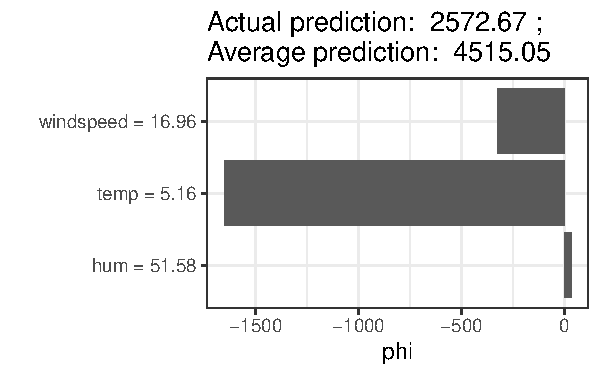
\includegraphics[width=\linewidth]{figure/shapley2shap.pdf}
% \end{column}
% \end{columns}
% 
% $$\Rightarrow
% \phi_{hum} = \tfrac{2}{6} (4635-4515) + \tfrac{1}{6} (3060-3087) + \tfrac{1}{6} (4450-4359) + \tfrac{2}{6} (2573-2623) = 34
% $$
% $\Rightarrow$ Analogously $\phi_{\text{temp}} = -1654$, $\phi_{\text{ws}} = -322$
% % \begin{align*}
% %  v(P) &= \fh(\xv) - \E(\fh) = \phi_{\text{hum}} + \phi_{\text{temp}} + \phi_{\text{ws}} \\
% %  &= {\color{orange} 2573} - {\color{blue} 4515} = 34 - 1654 - 322 = -1942
% %  \end{align*}
% 
% \medskip
% 
% \textbf{Interpretation:} \texttt{hum} raises prediction by 34, \texttt{temp} and \texttt{ws} lower it by 1654 and 322, explaining the deviation from the mean
% 
% %\textbf{Recall:} Shapley values explain how features shift prediction from baseline $\E(\fh)$:
% % \begin{align*}
% % v(P) &= \fh(\xv) - \E(\fh) = \phi_{\text{hum}} + \phi_{\text{temp}} + \phi_{\text{ws}} \\
% % &= {\color{orange} 2573} - {\color{blue} 4515} = 34 - 1654 - 322 = -1942
% % \end{align*}
% 
% \end{frame}



\begin{frame}{Shapley Values in ML - Example}
  
  \textbf{Example (Bike sharing data):}

  \begin{itemize}
  \item Train random forest using humidity (hum), temperature (temp), windspeed (ws)
      \item Consider observation of interest $\xv$ with prediction $\fh(\xv) = \color{orange}{2573}$
      \item Mean prediction $\E_{\xv}[\fh(\xv)] = \color{blue}{4515}$
      \item Compute exact Shapley value for $\xv$ for feature hum:
  \end{itemize}
  
      \begin{center}
      \begin{tabular}{c|c|c|c|c}
   $S$    &  $\Scupj$  & $\fh_S$ &  $\fh_{\Scupj}$  & weight\\\hline
     $\varnothing$&    hum  & \color{blue}{4515} & 4635 & $2/6$\\
       temp &  temp, hum & 3087 & 3060& $1/6$\\
       ws &  ws, hum & 4359  & 4450 & $1/6$\\
       temp, ws & temp, ws, hum & 2623 & \color{orange}{2573} & $2/6$
      \end{tabular}
      \end{center}
$$\Rightarrow
\phi_{\text{hum}}(\xv) = \tfrac{2}{6} (4635-4515) + \tfrac{1}{6} (3060-3087) + \tfrac{1}{6} (4450-4359) + \tfrac{2}{6} (2573-2623) = 34
$$
$\Rightarrow$ Analogously $\phi_{\text{temp}}(\xv) = -1654$, $\phi_{\text{ws}}(\xv) = -322$
% \begin{align*}
%  v(P) &= \fh(\xv) - \E(\fh) = \phi_{\text{hum}} + \phi_{\text{temp}} + \phi_{\text{ws}} \\
%  &= {\color{orange} 2573} - {\color{blue} 4515} = 34 - 1654 - 322 = -1942
%  \end{align*}

\end{frame}

% 
% \begin{frame}{From Shapley to SHAP}
% \textbf{Example continued}: Same calculation can be done for temperature and windspeed:
% \begin{itemize}
%     \item $\phi_{temp} = \ldots = -1654$
%     \item $\phi_{ws} = \ldots = -322$
% \end{itemize}
% 
% \textbf{Remember}: Shapley values explain difference between actual and average pred.:
% \begin{eqnarray*}
% \color{orange}{2573} \color{black}- \color{blue}{4515} \color{black} &= 34 - 1654 - 322 &= - 1942\\
% \fh(\xv) - \E(\fh) &= \phi_{hum} + \phi_{temp} + \phi_{ws}&\\
% \end{eqnarray*}
% \begin{columns}[T]
% \begin{column}{0.5\textwidth}
% $\leadsto$ can be rewritten as
% $$
% \fh(\xv) = \underbrace{\E(\fh)}_{\phi_0} + \phi_{hum} + \phi_{temp} + \phi_{ws}
% $$
% $\leadsto$ Additive decomposition: baseline $\phi_0$ + per-feature contributions $\phi_j$
% %N.B.: This reminds us of a LM with weights $\phi_j$ multiplied by a binary feature value indicating weather a feature is included in a considered coalition.
% \end{column}
% \begin{column}{0.5\textwidth}
% \vspace{-1cm}
% \begin{figure}
%     \centering
%     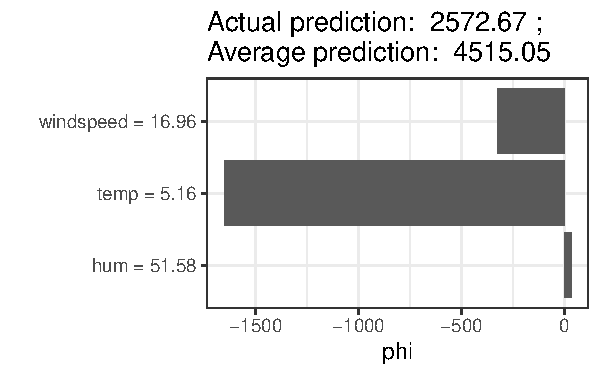
\includegraphics[width=0.9\columnwidth]{figure/shapley2shap.pdf}
% \end{figure}
% \end{column}
% \end{columns}
% \end{frame}

\begin{frame}{From Shapley Values to SHAP}


\begin{columns}[T, onlytextwidth]
\begin{column}{0.51\textwidth}

%\textbf{Example (cont.):} Shapley values for other features $\phi_{\text{temp}} = -1654$, $\phi_{\text{ws}} = -322$

%\medskip

% \textbf{Interpretation:} \texttt{hum} raises prediction by 34, \texttt{temp} and \texttt{ws} lower it by 1654 and 322, explaining the deviation from the mean

% \medskip
\textbf{Shapley value interpretation (for $\xv$):}
\begin{itemize}
  \item \texttt{hum}\(\;(+34)\) pushes pred. \emph{above} baseline (= average prediction).  
  \item \texttt{temp} \(\;(-1654)\) and \texttt{ws} \(\;(-322)\) pull prediction \emph{below} baseline.
  \item Together, they explain full deviation from average prediction.
\end{itemize}

%\medskip


% \textbf{Recall:} Shapley values explain how features shift prediction from baseline $\E(\fh)$:
% \footnotesize
% \begin{align*}
%  \fh(\xv) - \E_{\xv}[\fh(\xv)] &= \phi_{\text{hum}}(\xv) + \phi_{\text{temp}}(\xv)  + \phi_{\text{ws}}(\xv) \\
%  {\color{orange} 2573} - {\color{blue} 4515} &= 34 - 1654 - 322 = -1942
% \end{align*}

\end{column}
\begin{column}{0.49\textwidth}
%\vspace{-1cm}
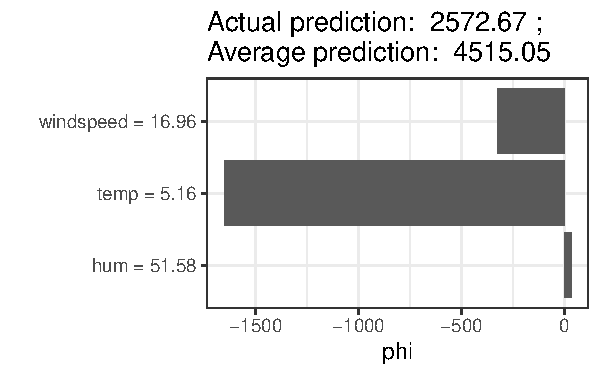
\includegraphics[trim={10 17 5 5},clip, width=\linewidth]{figure/shapley2shap.pdf}
\end{column}
\end{columns}
\pause
\textbf{Shapley-based additive decomposition} of prediction for $\xv$ gives insights on how features shift prediction from baseline $\E(\fh)$:

\medskip

\centerline{$
\underbrace{{\color{orange} \fh(\xv)}}_{\text{actual prediction}}
={\color{blue} \underbrace{\phi_0}_{\E_{\mathbf X}[\fh(\mathbf X)]}}
+\sum_{j\in\{\text{hum},\text{temp},\text{ws}\}}\phi_j(\xv)
$}
%\footnotesize
\medskip
\centerline{$
\phantom{=} \; {\color{orange} 2573}
= {\color{blue} 4515}
\;+\;
\bigl(34 -1654 - 322\bigr)
\;=\;4515-1942
$}
\medskip

\(\leadsto\) Like a LM evaluated at \(\xv\): global intercept \(\phi_0\) plus per-feature contribs \(\phi_j(\xv)\).

\medskip
%\vspace{0.4em}
% \textbf{SHAP:} Express prediction of $\xv$ as additive decomposition of Shapley values
% \[
% \fh(\xv) = \underbrace{\E(\fh)}_{\phi_0} + \sum_j \phi_j
% \]
% $\leadsto$ Analogous to linear models: intercept $\phi_0$ + per-feature contributions $\phi_j$

% \textbf{SHAP takeaway:}  
% \[
% \fh(\xv)=\underbrace{\E_{\xv}[\fh(\xv)]}_{\phi_0}
%       +\sum_{j=1}^{p}\phi_j(\xv)
%       \quad\text{with each }\phi_j(\xv)\text{ the \emph{Shapley value} of feature }j.
% \]

%\(\leadsto\) Like a linear model evaluated at \(\xv\): global intercept \(\phi_0\) plus instance-specific feature contributions \(\phi_j(\xv)\).

\textbf{SHAP Motivation:}
Can we efficiently estimate this Shapley-based additive decomp. of $\fh(\xv)$ via a surrogate model (while preserving Shapley axioms)?

%Additive explanation model: intercept $\phi_0$ plus per-feature effects $\phi_j$ (analogous to a linear model)
%Reminds of linear models: $\phi_j$ as effect of feature $j$ and intercept $\phi_0$ 
\end{frame}



% 
% \begin{frame}{From Shapley Values to the SHAP}
% 
% SHAP defines an \textbf{additive local surrogate model} \(g(\mathbf{z}^{\prime})\) based on a binary \textbf{simplified input} \(\mathbf{z}^{\prime} = (z^{\prime}_1, \dots, z^{\prime}_p)^\top \in \{0,1\}^p\), where:
% \[
% g(\mathbf{z}^{\prime}) = \phi_0 + \sum_{j=1}^p \phi_j z^{\prime}_j
% \]
% \begin{itemize}
%   \item \(z^{\prime}_j = 1\): feature \(j\) is "observed" (i.e., present in coalition)
%   \item \(z^{\prime}_j = 0\): feature \(j\) is "absent" and replaced via (conditional) imputation
%   \item SHAP seeks \(\phi_j\) values such that Shapley axioms hold %$\Rightarrow$ guarantees fairness, consistency, and efficiency.
% \end{itemize}
% \end{frame}
% % 
% % \begin{frame}{From Shapley to SHAP Model}
% % 
% % SHAP defines an additive feature attribution model (local surrogate model) \(g(\mathbf{z}^{\prime})\) based on a simplified feature vector \(\mathbf{z}^{\prime}\in\{0,1\}^p\) indicating whether a feature value was replaced by random imputation:
% % \[
% %  g(\mathbf{z}^{\prime})=\phi_0+\sum_{j=1}^p\phi_j z^{\prime}_j
% % \]
% % \begin{itemize}
% %   \item $z^{\prime}_j=1$ feature present; $z^{\prime}_j = 0$ replaced by random imputation.
% %   \item Find coefficients \(\phi_j\) such that Shapley axioms hold \(\Rightarrow\) SHAP.
% % \end{itemize}
% % \end{frame}
% 
% 
% \begin{frame}{SHAP Definition \furtherreading{LUNDBERG2017}}
% \textbf{Aim}: 
% %Find an additive combination that explains the prediction of an observation $\xv$ by computing the contribution of each feature to the prediction using a (more efficient) estimation procedure. \\\medskip
% Explain a prediction $\fh(\xv)$ by decomposing it into additive contributions from individual features using a surrogate model and efficient Shapley estimation.
% 
% \medskip
% 
% \only<1-5>{\textbf{SHAP Setup}
% \begin{itemize}
%     % \item Simplified (binary) coalition feat. space $\mathbf{Z}^\prime \in \{0,1\}^{K \times p}$ with $K$ rows and $p$ cols.
%     % \item Rows are referred to as $\mathbf{z}^{\prime (k)} = \{z^{\prime (k)}_1, \ldots, z^{\prime (k)}_p\}$ with $k \in \{1,\ldots, K\}$ (indexes $k$-th coalition)
%     % \item Cols are referred to as $\mathbf{z}_j$ with $j \in \{1, \ldots, p\}$ being the index of the original feat.
%      \item Simplified (binary) coalition feat. space $\mathbf{Z}^\prime \in \{0,1\}^{K \times p}$ with $K$ rows and $p$ cols.
%     \item Each row $\mathbf{z}^{\prime (k)} = (z_1^{\prime(k)}, \ldots, z_p^{\prime(k)})$ represents a coalition (subset of features).
%     \item Each column $\mathbf{z}_j$ indicates if feature $j$ is part of a coalition.
% \end{itemize}
% }
% 
% \medskip
% 
% \only<1>{
% \textbf{Example -- Coalition Space for 3 Features}: 
% \vspace{-0.2cm}
% \begin{table}[]
%     \centering
%     \footnotesize
%      \begin{tabular}{l |c|ccc}
%   Coalition  & $\mathbf{z}^{\prime (k)}$ &  hum & temp & ws \\
%   \hline 
%   $\varnothing$ & $\mathbf{z}^{\prime (1)}$ & 0 & 0 & 0  \\
%   hum & $\mathbf{z}^{\prime (2)}$ & 1 & 0 & 0  \\
%   temp &  $\mathbf{z}^{\prime (3)}$ & 0 & 1 & 0  \\
%   ws &   $\mathbf{z}^{\prime (4)}$ & 0 & 0 & 1  \\
%   hum, temp & $\mathbf{z}^{\prime (5)}$ & 1 & 1 & 0  \\
%   temp, ws & $\mathbf{z}^{\prime (6)}$ & 0 & 1 & 1  \\
%   hum, ws &   $\mathbf{z}^{\prime (7)}$ & 1 & 0 & 1  \\
%   hum, temp, ws & $\mathbf{z}^{\prime (8)}$ & 1 & 1 & 1  \\
%   \end{tabular}
% \end{table}
% }
% \only<2->{
% %\vspace{0.5cm}
% \begin{exampleblock}{}
% \[
% g\left(\tikzmark{zp} \mathbf{z}^{\prime (k)}\right)=
% \tikzmark{ph0}\phi_{0}+\sum_{j=1}^{p}
% \tikzmark{phj} \phi_{j} z_{j}^{\prime (k)}
% \]
% \begin{tikzpicture}[
%   remember picture,
%   overlay,
%   expl/.style={draw=blue,fill=white,rounded corners,text width=3cm},
%   arrow/.style={blue,ultra thick,->,>=latex}
% ]
% \node<2-4>[expl] 
%   (zex) 
%   at (2,1.5cm)
%   {$\mathbf{z}^{\prime (k)}$: \textbf{Coalition} \\ simplified features};
% \node<3-4>[expl] 
%   (ph0ex) 
%   at (4,-.5cm)
%   {$\phi_0$: \textbf{Null Output} \\ Average Model Baseline ($\E(\fh))$};
% \node<4>[expl] 
%   (phjex) 
%   at (10,0cm)
%   {$\phi_j$: \textbf{Attribution} \\ How much does feature $j$ change the output for coalition $k$};
% 
% \draw<2-4>[arrow]
%   (zex.east) to[out=0,in=120] ([xshift= 1ex, yshift=2.3ex]{pic cs:zp});  
% \draw<3-4>[arrow]
%   (ph0ex.east) to[out=0,in=270] ([xshift= 1ex, yshift=-0.8ex]{pic cs:ph0});  
% \draw<4>[arrow]
%   (phjex.west) to[out=180,in=270] ([xshift= 1ex, yshift=-1ex]{pic cs:phj});
%  \node<5>[expl] 
%   (zex)  
%   at (2,1cm)
%   {$g(\mathbf{z}^{\prime (k)})$: \textbf{Marginal Contribution} \\ Contribution of coalition $\mathbf{z}^{\prime (k)}$ to the prediction};
%   \draw<5>[arrow]
%   (zex.east) to[out=0,in=140] ([xshift= 1ex, yshift=2.3ex]{pic cs:zp});  
% \node<5>[expl] 
%   (phjsh) 
%   at (10,1.5cm)
%   {$\phi_j$: \textbf{Shapley Values}};
% \draw<5>[arrow]
%   (phjsh.west) to[out=180,in=50] ([xshift= 1ex, yshift=2ex]{pic cs:phj}); 
% \draw<5> [
%     thick,
%     decoration={
%         brace,
%         mirror,
%         raise=0.5cm
%     },
%     decorate
% ] (5.7,0.7) -- (8.2,0.7)
% node[pos=0.5,below=15pt,black]{\textbf{Additive Feature Attribution}};
% \end{tikzpicture}
% \end{exampleblock}
% \begin{onlyenv}<5>
% \vspace{1cm}
% \textbf{Next:} How do we estimate the Shapley values $\phi_j$ efficiently?
% \end{onlyenv}}
% 
% \end{frame}

\begin{frame}{SHAP Framework \furtherreading{LUNDBERG2017}}

\textbf{SHAP} expresses the prediction of $\xv$ as a sum of contribs from each feature:

\[
g(\zv') = \phi_0 + \textstyle\sum_{j=1}^p \phi_j z'_j
\]

\begin{itemize}
  \item $\zv' \in \{0,1\}^p$: simplified binary input referring to a coalition (coal. vector)
  \item \(z'_j = 1\): feature $j$ is "present" $\Rightarrow$ use $x_j$ in model evaluation
  \item \(z'_j = 0\): feature $j$ is "absent"\\$\Rightarrow$ influence of $x_j$ is removed via marginalization over a reference distrib.% (averaging predictions over its possible values, given the present features)%\\
  %$\leadsto$ \textit{Note: In practice (e.g., KernelSHAP), marginalization is approximated via random imputations from background data.}
\end{itemize}

\pause\medskip

\textbf{SHAP as a theoretical framework:} Fit a surrogate model \( g(\zv') \) satisfying Shapley axioms and recovering $\fh(\xv)$ when all features are "present":
%Construct a surrogate model $g(\zv')$ such that it satisfies the Shapley value axioms and recovers $\fh(\xv)$ when all features are "present":
\[
\fh(\xv) = g(\mathbf{1}) = \phi_0 + \textstyle\sum_{j=1}^p \phi_j
\]
\textbf{Evaluation of $g(\zv')$:} Let \( S = \{ j : z'_j = 1 \} \) be the active coalition. Then:
\begin{itemize}
    \item $g(\zv') \approx \mathbb{E}[ \fh(\mathbf{X}) \mid \mathbf{X}_S = \mathbf{x}_S]\;\text{(conditional expectation)}$
    \item $g(\zv') \approx \mathbb{E}_{\mathbf{X}_{-S}} [ \fh(\mathbf{x}_S, \mathbf{X}_{-S}) ] \;\;\text{(marginal expectation, i.e., PD function)}$
    \item\textit{Note: Practical implementations (e.g., KernelSHAP) use the marginal expectation, approximated via random imputations from background data.}
\end{itemize}

\end{frame}


% \begin{frame}{SHAP Framework \furtherreading{LUNDBERG2017}}

% \textbf{SHAP} expresses the prediction of $\xv$ as a sum of contributions from each feature:

% \[
% g(\zv') = \phi_0 + \sum_{j=1}^p \phi_j z'_j
% \]

% \begin{itemize}
%   \item $\zv' \in \{0,1\}^p$: simplified binary input referring to a coalition (coalition vector)
%   \item \(z'_j = 1\): feature $j$ is "present" $\Rightarrow$ use $x_j$ in the model evaluation
%   \item \(z'_j = 0\): feature $j$ is "absent" $\Rightarrow$ marginalize $x_j$ (average over its possible values)\\
%   $\leadsto$ \textit{Note: In practice (e.g., KernelSHAP), marginalization is approximated via random imputations from background data.}
% \end{itemize}

% \vspace{0.5em}
% \textbf{Key idea:} Construct a surrogate model $g(\zv')$ such that it satisfies the Shapley value axioms and recovers $\fh(\xv)$:
% \[
% \fh(\xv) = g(\mathbf{1}) = \phi_0 + \sum_{j=1}^p \phi_j
% \]


% \end{frame}


% \begin{frame}{SHAP Framework \furtherreading{LUNDBERG2017}}

% \textbf{SHAP} defines a surrogate \(g(\zv')\) over binary vectors \(\zv' \in \{0,1\}^p\) (simplified features):

% \[
% g(\zv') = \phi_0 + \sum_{j=1}^p \phi_j z'_j
% \]

% \begin{itemize}

%   \item \textbf{Fixed:} \(\xv\) is the instance being explained (i.e., SHAP explains \(\fh(\xv)\))
%   \item \textbf{Coalitions:} \(\zv'\) encodes which features of \(\xv\) are "observed" in coalition:
%     \begin{itemize}
%       \item \(z'_j = 1\): feature \(j\) is included $\Rightarrow$ use \(x_j\)
%       \item \(z'_j = 0\): feature \(j\) is excluded $\Rightarrow$ \(x_j\) is marginalized out
%       %random imputation when evaluating \(\fh\)
%     \end{itemize}
% \item Each $\zv'$ represents a \textbf{feature coalition} used to approximate $\fh(\xv)$\\
% %Each \(\zv'\) represents a \textbf{coalition}, i.e., a subset of features considered "known" for the prediction at \(\xv\)
%   %\item Many different \(\zv'\) are used for the same \(\xv\), to simulate all possible feature subsets and compute marginal contributions.
%   $\leadsto$ Many \(\zv'\) are constructed from \(\xv\), defining a subset of "observed" features\\
%   $\leadsto$ Used to estimate marginal contributions and compute Shapley values
%   \item SHAP computes \(\phi_j\) such that \(g(\zv')\) satisfies Shapley axioms and recovers \(\fh(\xv)\)
%   %SHAP chooses the \(\phi_j\) such that \(g(\zv')\) approximates \(\fh(\xv)\) in a way that satisfies the Shapley axioms.
% \end{itemize}


%  \end{frame}

\begin{frame}{SHAP Framework \furtherreading{LUNDBERG2017}}

%\textbf{Goal:} Explain a prediction \(\fh(\xv)\) by decomposing it into additive feature contributions using a local surrogate model derived from Shapley values.

\medskip

\textbf{SHAP}  
defines an additive surrogate \(g(\zv')\) over a binary input \(\zv' \in \{0,1\}^p\):
% \only<1>{
% \[
% g(\zv') = \phi_0 + \sum_{j=1}^p \phi_j z'_j
% \]
% \begin{itemize}
%   \item \(z'_j = 1\): feature \(j\) is "observed" (included in coalition)
%   \item \(z'_j = 0\): feature \(j\) is "absent" and replaced via (conditional) imputation
%   \item \(\phi_j\): contribution of feature \(j\) to \(\fh(\xv)\), satisfying Shapley axioms
% \end{itemize}

% \medskip

% \textbf{Coalition space:} each row \(\zv'^{(k)} \in \{0,1\}^p\) refers to a coalition

% \begin{table}[]
%     \centering
%     \footnotesize
%      \begin{tabular}{l |c|ccc}
%   Coalition  & $\zv'^{(k)}$ &  hum & temp & ws \\
%   \hline 
%   $\varnothing$ & $\zv'^{(1)}$ & 0 & 0 & 0  \\
%   hum & $\zv'^{(2)}$ & 1 & 0 & 0  \\
%   temp &  $\zv'^{(3)}$ & 0 & 1 & 0  \\
%   ws &   $\zv'^{(4)}$ & 0 & 0 & 1  \\
%   hum, temp & $\zv'^{(5)}$ & 1 & 1 & 0  \\
%   temp, ws & $\zv'^{(6)}$ & 0 & 1 & 1  \\
%   hum, ws &   $\zv'^{(7)}$ & 1 & 0 & 1  \\
%   hum, temp, ws & $\zv'^{(8)}$ & 1 & 1 & 1  \\
%   \end{tabular}
% \end{table}
% }

\only<1->{
\begin{exampleblock}{}
\[
g\left(\tikzmark{zp} \zv'^{(k)}\right) =
\tikzmark{ph0} \phi_0 + \sum_{j=1}^p \tikzmark{phj} \phi_j z_j'^{(k)}
\]
\begin{tikzpicture}[
  remember picture,
  overlay,
  expl/.style={draw=blue,fill=white,rounded corners,text width=3.5cm},
  arrow/.style={blue,ultra thick,->,>=latex}
]
\node<1>[expl] (zex) at (2,1.5cm)
  {\(\zv'^{(k)}\): \textbf{coalition vector} \\ subset of features};
\node<1>[expl] (ph0ex) at (4,-.5cm)
  {\(\phi_0\): \textbf{baseline} \(\E[\fh(\Xv)]\)};
\node<1>[expl] (phjex) at (10,0cm)
  {\(\phi_j\): \textbf{feature attribution} \\ marginal effect of \(j\) in coalition};

\draw<1>[arrow] (zex.east) to[out=0,in=120] ([xshift= 1ex, yshift=2.3ex]{pic cs:zp});  
\draw<1>[arrow] (ph0ex.east) to[out=0,in=270] ([xshift= 1ex, yshift=-0.8ex]{pic cs:ph0});  
\draw<1>[arrow] (phjex.west) to[out=180,in=270] ([xshift= 1ex, yshift=-1ex]{pic cs:phj});

\node<2>[expl] (zex2) at (2,1cm)
  {\(g(\zv'^{(k)})\): \textbf{approx. prediction} for coalition};
\draw<2>[arrow] (zex2.east) to[out=0,in=140] ([xshift= 1ex, yshift=2.3ex]{pic cs:zp});  
\node<2>[expl] (phjsh) at (10,1.5cm)
  {\(\phi_j\): \textbf{Shapley value}};
\draw<2>[arrow] (phjsh.west) to[out=180,in=50] ([xshift= 1ex, yshift=2ex]{pic cs:phj}); 
\draw<2>[thick, decoration={brace, mirror, raise=0.5cm}, decorate]
  (5.7,0.7) -- (8.2,0.7)
  node[pos=0.5,below=15pt,black]{\textbf{Additive Feature Attribution}};
\end{tikzpicture}
\end{exampleblock}

\begin{onlyenv}<2>
\vspace{1cm}
\textbf{Next:} How do we estimate the Shapley values \(\phi_j\) efficiently?
\end{onlyenv}
}
\end{frame}


%\begin{frame}{Example}

%Given the following example from the bike sharing data set

%\begin{table}[h]
%\centering
%\begin{tabular}{l rrrrr || r}
%  \hline
%  && temperature & humidity & windspeed & year & prediction\\ 
%  \hline
% example $x_{ex}$ && 24.27 & 58.5 & 13.96 & 2011 & 6825 \\ 
% \hline
%\end{tabular}
%\end{table}

%we are searching for Shapley values such that
%\begin{equation}
%\begin{array}{lllllcr}
%\phi_0 &+ \phi_{temp} &+ \phi_{hum} &+ \phi_{windspeed} &+ \phi_{yr} & = &\hat{y} \\
%4469 &+ 1809 &+ 450 &+ 241 &- 144 & = & 6825
%\end{array}
%\end{equation}

%\begin{figure}
 %   \centering
 %   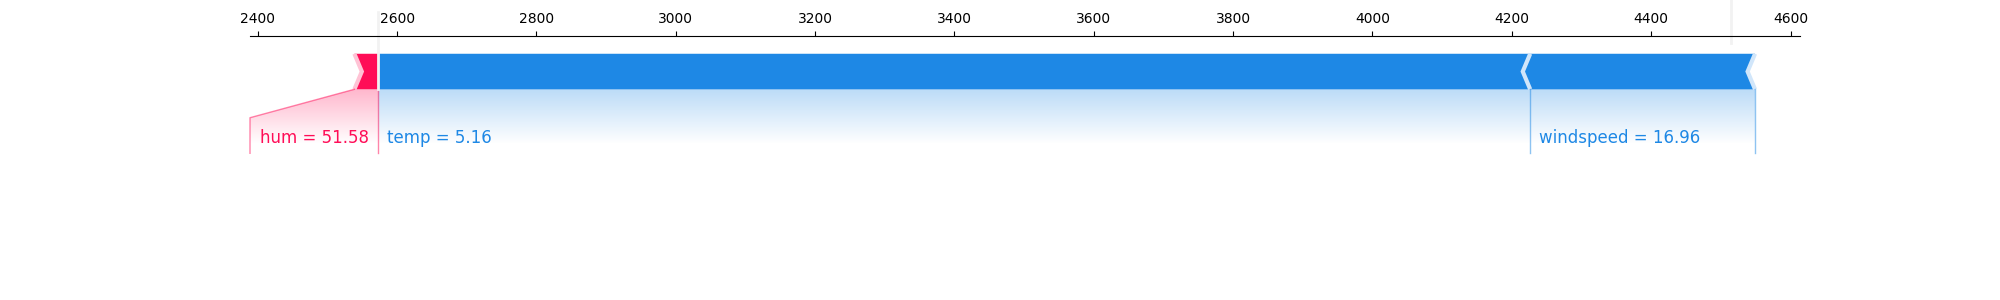
\includegraphics[width=\columnwidth]{figure_man/exSHAP.png}
%\end{figure}
%\end{frame}


\begin{frame}{Properties}

\textbf{Local Accuracy}
$$
\fh(\xv)=g\left(\mathbf{z}^{\prime}\right)=\phi_{0}+\sum_{j=1}^{p} \phi_{j} z_{j}^{\prime}
$$

\begin{onlyenv}<1>
\textbf{Intuition:} If coalition includes all features ($\mathbf{z}^{\prime} = (z^{\prime}_1, \dots, z^{\prime}_p)^\top = (1, \dots, 1)^\top $), the attributions $\phi_j$ and the baseline $\phi_0$ sum up to the original model output $\fh(\xv)$\\\medskip
Local accuracy corresponds to \textbf{axiom of efficiency} in Shapley game theory

\end{onlyenv}

\begin{onlyenv}<2->
\textbf{Missingness}
$$
z_{j}^{\prime}=0 \Longrightarrow \phi_{j}=0
$$
\end{onlyenv}

\begin{onlyenv}<2>
\textbf{Intuition:}  A "missing" feature (whose value is imputed) gets zero attribution 
\end{onlyenv}

\begin{onlyenv}<3->
\textbf{Consistency} (Let $\mathbf{z}^{\prime (k)}_{-j} \text{ refer to } z_{j}^{\prime (k)}=0$) \\
\end{onlyenv}

\begin{onlyenv}<3>
For any two models $\fh$ and $\fh^{\prime}$, if for all inputs $\mathbf{z}^{\prime (k)} \in \{0, 1\}^p$

$$
\fh_{x}^{\prime}\left(\mathbf{z}^{\prime (k)}\right)-\fh_{x}^{\prime}\left(\mathbf{z}^{\prime (k)}_{-j}\right) \geq \fh_{x}\left(\mathbf{z}^{\prime (k)}\right)-\fh_{x}\left(\mathbf{z}^{\prime (k)} _{-j}\right) \Longrightarrow \phi_{j}\left(\fh^{\prime}, \xv\right) \geq \phi_{j}(\fh, \xv)
$$

\textbf{Intution:} If a model changes so that the marginal contribution of a feature value increases or stays the same, the Shapley value also increases or stays the same\\\medskip
\textbf{Consistency} implies Shapley’s axioms of \textbf{additivity, dummy, symmetry}.
\end{onlyenv}


\end{frame}

\endlecture
\end{document}
